% Source of the figure two-color-examples.pdf: (a) the cubic 3-connected plane graph with 14 vertices and
% 21 edges that has no [2,2]-edge coloring, (b) the 3-connected plane graph with 11 vertices and 18 edges
% that has no [1,3]-edge coloring. Vertex numbers are those of the rotation systems C21 and D18 in the
% file examples.json of the checks. Compile with pdfLaTeX; the PDF is included at its natural size.
\documentclass[tikz,border=1pt]{standalone}
\usepackage[T1]{fontenc}
\usepackage{lmodern}
\pdfinfoomitdate=1 \pdftrailerid{} \pdfsuppressptexinfo=-1
\tikzset{
  vertex/.style={circle, fill=black, inner sep=0pt, minimum size=1.9mm},
  edge/.style={line width=0.7pt}}
\begin{document}
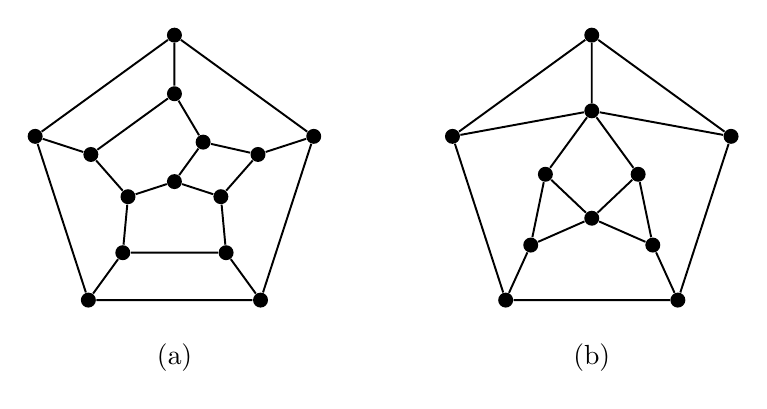
\begin{tikzpicture}[x=0.62cm, y=0.62cm]
  % (a) outer pentagon 0,1,9,8,3; octagon 2,10,13,7,5,6,4,11; centre 12
  \begin{scope}
    \node[vertex] (a0)  at (90:3)     {};
    \node[vertex] (a1)  at (162:3)    {};
    \node[vertex] (a9)  at (234:3)    {};
    \node[vertex] (a8)  at (306:3)    {};
    \node[vertex] (a3)  at (18:3)     {};
    \node[vertex] (a2)  at (90:1.8)   {};
    \node[vertex] (a10) at (162:1.8)  {};
    \node[vertex] (a13) at (198:1.0)  {};
    \node[vertex] (a7)  at (234:1.8)  {};
    \node[vertex] (a5)  at (306:1.8)  {};
    \node[vertex] (a6)  at (342:1.0)  {};
    \node[vertex] (a4)  at (18:1.8)   {};
    \node[vertex] (a11) at (54:1.0)   {};
    \node[vertex] (a12) at (0,0)      {};
    \draw[edge] (a0) -- (a1) (a0) -- (a2) (a3) -- (a4) (a5) -- (a6) (a5) -- (a7) (a8) -- (a9) (a1) -- (a10)
                (a11) -- (a4) (a4) -- (a6) (a12) -- (a13) (a7) -- (a9) (a9) -- (a1) (a11) -- (a12)
                (a10) -- (a13) (a3) -- (a0) (a11) -- (a2) (a2) -- (a10) (a8) -- (a5) (a3) -- (a8)
                (a12) -- (a6) (a7) -- (a13);
    \node at (0,-3.6) {(a)};
  \end{scope}
  % (b) outer pentagon 1,2,10,9,7; vertex 0 of degree five; vertex 5 of degree four
  \begin{scope}[xshift=5.3cm]
    \node[vertex] (b1)  at (90:3)        {};
    \node[vertex] (b2)  at (162:3)       {};
    \node[vertex] (b10) at (234:3)       {};
    \node[vertex] (b9)  at (306:3)       {};
    \node[vertex] (b7)  at (18:3)        {};
    \node[vertex] (b0)  at (0,1.45)      {};
    \node[vertex] (b3)  at (-0.95,0.15)  {};
    \node[vertex] (b4)  at (0.95,0.15)   {};
    \node[vertex] (b5)  at (0,-0.75)     {};
    \node[vertex] (b8)  at (-1.25,-1.3)  {};
    \node[vertex] (b6)  at (1.25,-1.3)   {};
    \draw[edge] (b0) -- (b1) (b0) -- (b2) (b0) -- (b3) (b4) -- (b5) (b4) -- (b6) (b0) -- (b7) (b1) -- (b2)
                (b8) -- (b3) (b3) -- (b5) (b5) -- (b6) (b9) -- (b7) (b7) -- (b1) (b8) -- (b5) (b10) -- (b9)
                (b0) -- (b4) (b10) -- (b2) (b9) -- (b6) (b8) -- (b10);
    \node at (0,-3.6) {(b)};
  \end{scope}
\end{tikzpicture}
\end{document}
